\section{去重：从精确重复到近重复}

\subsection{为什么去重要单独讲}

过滤解决的是“留下什么”，去重解决的是“别重复留下什么”。它特别重要，因为重复数据会导致训练效率下降、记忆化上升，甚至引入版权和隐私问题。课程里把去重分成精确重复和近重复两类，这个划分非常关键。

\begin{figure}[H]
\centering
\begin{tikzpicture}[node distance=1.0cm, every node/.style={font=\small, align=center}]
\node[draw, rounded corners, fill=green!10, minimum width=3cm, minimum height=0.85cm] (exact) {exact duplicate};
\node[draw, rounded corners, fill=yellow!16, below=of exact, minimum width=3cm, minimum height=0.85cm] (near) {near duplicate};
\node[draw, rounded corners, fill=red!10, below=of near, minimum width=3cm, minimum height=0.85cm] (hard) {hard at scale};
\draw[-{Latex[length=3mm]}, thick] (exact) -- (near);
\draw[-{Latex[length=3mm]}, thick] (near) -- (hard);
\end{tikzpicture}
\caption{去重从精确重复走向近重复后，问题会迅速从“简单 hash”升级为“可扩展的相似度检索”}
\end{figure}

\subsection{精确重复}

精确重复最简单：按 hash 分组，每组留一个。MapReduce 风格天然适合这个任务，因为你可以先局部 hash，再全局 merge。C4 常见的做法是以 3-sentence span 为单位做精确去重，简单但有效。

\begin{figure}[H]
\centering
\begin{tikzpicture}[every node/.style={font=\small, align=center}]
\node[draw, rounded corners, fill=blue!10, minimum width=2.8cm, minimum height=0.85cm] (a) at (0,2.0) {A: hello};
\node[draw, rounded corners, fill=blue!10, minimum width=2.8cm, minimum height=0.85cm] (b) at (0,0.6) {B: hello};
\node[draw, rounded corners, fill=blue!10, minimum width=2.8cm, minimum height=0.85cm] (c) at (0,-0.8) {C: hi};
\node[draw, rounded corners, fill=blue!10, minimum width=2.8cm, minimum height=0.85cm] (d) at (0,-2.2) {D: bye};
\node[draw, rounded corners, fill=yellow!16, right=4.0cm of b, minimum width=3.4cm, minimum height=1.1cm] (bucket) {hash bucket\\{A,B} \; \{C\} \; \{D\}};
\draw[-{Latex[length=3mm]}, thick] (a) -- (bucket);
\draw[-{Latex[length=3mm]}, thick] (b) -- (bucket);
\draw[-{Latex[length=3mm]}, thick] (c) -- (bucket);
\draw[-{Latex[length=3mm]}, thick] (d) -- (bucket);
\end{tikzpicture}
\caption{精确去重的最小原型：把 hash 一样的样本分到同一桶里，每桶保留一个}
\end{figure}

\begin{importantbox}{精确去重的优点}
\begin{itemize}
    \item 语义清楚。
    \item 高精度。
    \item 非常容易并行化。
\end{itemize}
\end{importantbox}

\begin{warningbox}{精确去重的缺点}
它抓不住只差几个 token 的近重复，也可能把文档中间的一段切掉，导致剩余上下文不连贯。
\end{warningbox}

\subsection{Bloom filter}

Bloom filter 是一个典型的工程妥协：它用少量误报换大量空间节省。它适合快速判断“这个 item 有没有出现过”，但不适合精确删除。

\begin{figure}[H]
\centering
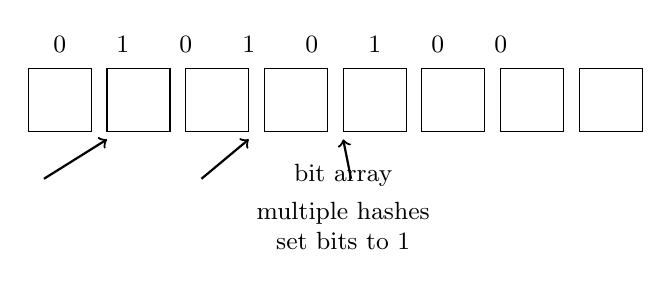
\begin{tikzpicture}[every node/.style={font=\small}]
\foreach \x in {0,...,7} {
  \draw (\x,0) rectangle ++(0.8,0.8);
}
\node at (0.4,1.1) {0};
\node at (1.2,1.1) {1};
\node at (2.0,1.1) {0};
\node at (2.8,1.1) {1};
\node at (3.6,1.1) {0};
\node at (4.4,1.1) {1};
\node at (5.2,1.1) {0};
\node at (6.0,1.1) {0};
\node at (4.0,-0.55) {bit array};
\draw[->, thick] (0.2,-0.6) -- (1.0,-0.1);
\draw[->, thick] (2.2,-0.6) -- (2.8,-0.1);
\draw[->, thick] (4.1,-0.6) -- (4.0,-0.1);
\node[align=center] at (4,-1.2) {multiple hashes\\set bits to 1};
\end{tikzpicture}
\caption{Bloom filter 的基本结构：若干哈希把元素映射到 bit array 上的多个位置}
\end{figure}

如果用 $m$ 个桶、$k$ 个哈希函数、插入 $n$ 个元素，假阳性率近似为
\[
f\approx \left(1-e^{-kn/m}\right)^k.
\]
在固定 $m/n$ 下，最优的 $k$ 大约是
\[
k\approx \frac{m}{n}\ln 2.
\]

\begin{figure}[H]
\centering
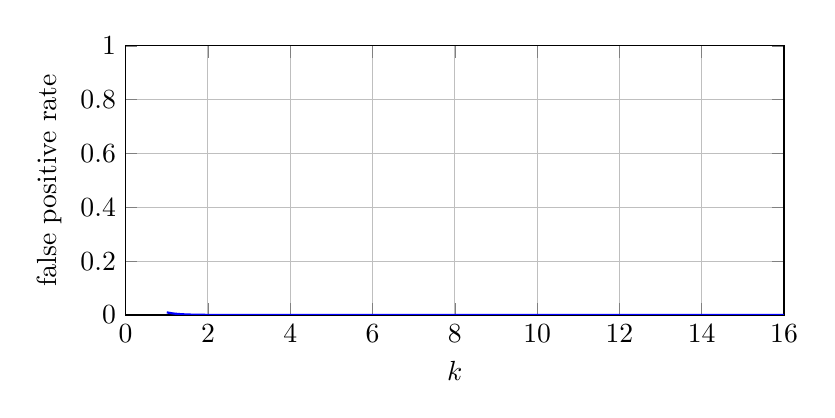
\begin{tikzpicture}
\begin{axis}[
    width=0.82\textwidth,
    height=5cm,
    xlabel={$k$},
    ylabel={false positive rate},
    ymin=0, ymax=1,
    xmin=0, xmax=16,
    grid=both,
]
\addplot[blue, thick, domain=1:16, samples=200] { (1 - exp(-10*x/1000))^x };
\end{axis}
\end{tikzpicture}
\caption{Bloom filter 的参数权衡：哈希函数越多，误报率先降后升，存在一个最优点}
\end{figure}

\begin{warningbox}{Bloom filter 的本质}
它不是要“绝对正确”，而是用少量误报换极低内存占用。对网页级去重来说，这通常是合理的。
\end{warningbox}

\subsection{Jaccard 和 MinHash}

近重复检测通常要先定义相似度。最常见的是 Jaccard：
\[
\mathrm{Jaccard}(A,B)=\frac{|A\cap B|}{|A\cup B|}.
\]
如果两个文档的 Jaccard 足够高，就可以把它们看成近重复候选。但难点在于：怎么不做全量两两比较。

\begin{figure}[H]
\centering
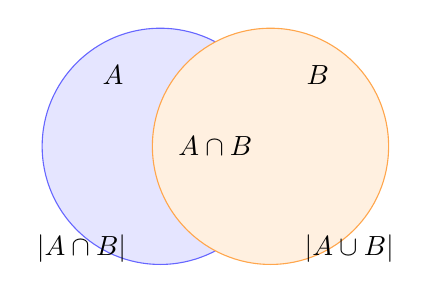
\begin{tikzpicture}[scale=1]
\draw[fill=blue!10, draw=blue!60] (0,0) circle (1.5);
\draw[fill=orange!12, draw=orange!70] (1.4,0) circle (1.5);
\node at (-0.6,0.9) {$A$};
\node at (2.0,0.9) {$B$};
\node at (0.7,0) {$A\cap B$};
\node at (-1.0,-1.3) {$|A\cap B|$};
\node at (2.4,-1.3) {$|A\cup B|$};
\end{tikzpicture}
\caption{Jaccard 的直觉：看两个集合的重叠程度，而不是单独看每个集合有多大}
\end{figure}

MinHash 的关键性质是：对于随机哈希函数 $h$，
\[
\Pr[h(A)=h(B)] = \mathrm{Jaccard}(A,B).
\]
这意味着你不用显式算所有集合相似度，只要看“是否碰撞”就能估计近重复关系。

\begin{figure}[H]
\centering
\begin{tikzpicture}[node distance=1.0cm, every node/.style={font=\small}]
\node[draw, rounded corners, fill=green!10, minimum width=2.2cm, minimum height=0.8cm] (s1) {set A};
\node[draw, rounded corners, fill=green!10, right=of s1, minimum width=2.2cm, minimum height=0.8cm] (s2) {set B};
\node[draw, rounded corners, fill=yellow!16, below=of s1, minimum width=2.2cm, minimum height=0.8cm] (perm) {random permutation};
\node[draw, rounded corners, fill=blue!14, below=of s2, minimum width=2.2cm, minimum height=0.8cm] (min) {first seen item};
\draw[-{Latex[length=3mm]}, thick] (s1) -- (perm);
\draw[-{Latex[length=3mm]}, thick] (s2) -- (perm);
\draw[-{Latex[length=3mm]}, thick] (perm) -- (min);
\node[below=0.8cm of perm, align=center] {相似集合更容易在同一位置“先出现”};
\end{tikzpicture}
\caption{MinHash 的直觉：把集合做随机排列，再看最先出现的元素是否一致}
\end{figure}

\begin{importantbox}{MinHash 的作用}
它把相似度问题变成了“碰撞概率”问题。概率一旦可估计，就能进一步用来做大规模索引和候选召回。
\end{importantbox}

\subsection{LSH：把概率差异放大成阈值效应}

LSH 的核心是 banding。把 $n$ 个 hash 分成 $b$ 个 band，每个 band 有 $r$ 个 hash，满足 $n=br$。若相似度为 $s$，那么某个 band 匹配的概率是 $s^r$，至少有一个 band 匹配的概率是
\[
1-(1-s^r)^b.
\]

\begin{figure}[H]
\centering
\begin{tikzpicture}[every node/.style={font=\small, align=center}]
\foreach \i in {0,...,7} {
  \draw (0,-0.8*\i) rectangle ++(2.8,0.55);
}
\draw[decorate, decoration={brace, amplitude=5pt}] (3.0,0) -- (3.0,-1.65);
\node[right=0.4cm of {$(3.0,-0.8)$}] {band 1};
\draw[decorate, decoration={brace, amplitude=5pt}] (3.0,-2.0) -- (3.0,-3.65);
\node[right=0.4cm of {$(3.0,-2.8)$}] {band 2};
\draw[decorate, decoration={brace, amplitude=5pt}] (3.0,-4.0) -- (3.0,-5.65);
\node[right=0.4cm of {$(3.0,-4.8)$}] {band 3};
\end{tikzpicture}
\caption{LSH 的 banding 思路：把多个 hash 分块，任何一块完全相同都能触发候选对}
\end{figure}

\begin{figure}[H]
\centering
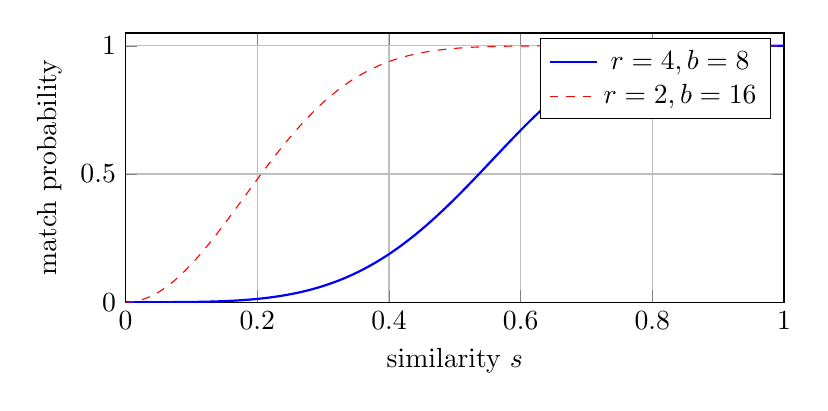
\begin{tikzpicture}
\begin{axis}[
    width=0.82\textwidth,
    height=5cm,
    xlabel={similarity $s$},
    ylabel={match probability},
    ymin=0, ymax=1.05,
    xmin=0, xmax=1,
    grid=both,
]
\addplot[blue, thick, domain=0:1, samples=120] {1 - (1 - x^4)^8};
\addplot[red, dashed, domain=0:1, samples=120] {1 - (1 - x^2)^16};
\addlegendentry{$r=4,b=8$}
\addlegendentry{$r=2,b=16$}
\end{axis}
\end{tikzpicture}
\caption{LSH 的阈值效应：不同 banding 参数会让曲线在不同相似度位置陡然上升}
\end{figure}

\begin{knowledgebox}{LSH 的工程意义}
\begin{itemize}
    \item 先哈希分桶，再做局部比较。
    \item 把连续相似度问题变成碰撞问题。
    \item 对大规模近重复召回非常合适。
\end{itemize}
\end{knowledgebox}

\subsection{shingle 选择与归一化}

MinHash 和 LSH 并不是直接对原始字符串做，而通常是先把文本切成 word shingles 或 character shingles，再做集合化表示。选择多少 token 一组，不是纯数学问题，而是对语言形态、编辑差异和噪声类型的折中。

\begin{table}[H]
\centering
\small
\renewcommand{\arraystretch}{1.15}
\begin{tabular}{p{2.8cm}p{4.4cm}p{4.0cm}}
\toprule
\textbf{shingle 类型} & \textbf{优点} & \textbf{缺点} \\
\midrule
word shingles & 更符合语义块 & 对标点和分词敏感 \\
char shingles & 对拼写和局部改写更稳 & 可能太细、噪声更多 \\
sentence spans & 适合整段去重 & 切分误差会放大 \\
\bottomrule
\end{tabular}
\caption{近重复检测里最先要想清楚的，不是算法，而是 shingle 怎么定义}
\end{table}

\begin{figure}[H]
\centering
\begin{tikzpicture}[every node/.style={font=\small, align=center}]
\node[draw, rounded corners, fill=blue!10, minimum width=3.5cm, minimum height=0.9cm] (a) {the cat sat on the mat};
\node[draw, rounded corners, fill=blue!10, below=of a, minimum width=3.5cm, minimum height=0.9cm] (b) {the cat sat on a mat};
\node[draw, rounded corners, fill=yellow!16, right=3.8cm of a, minimum width=3.6cm, minimum height=1.1cm] (sh) {shared shingles\\the cat / cat sat / sat on};
\draw[-{Latex[length=3mm]}, thick] (a) -- (sh);
\draw[-{Latex[length=3mm]}, thick] (b) -- (sh);
\node[below=0.8cm of b, align=center] {轻微改写后仍保留大量共享 shingle};
\end{tikzpicture}
\caption{近重复检测的直觉例子：只改一个词，仍然会留下足够多的共享片段}
\end{figure}

\subsection{LSH 参数怎么选}

LSH 的参数本质上在调召回和精度的分界线。$r$ 越大，单个 band 越严格；$b$ 越大，触发候选的机会越多。它们共同决定曲线在什么相似度附近拐起来。

\begin{table}[H]
\centering
\small
\renewcommand{\arraystretch}{1.15}
\begin{tabular}{p{2.4cm}p{4.1cm}p{4.0cm}p{3.0cm}}
\toprule
\textbf{参数变化} & \textbf{效果} & \textbf{代价} & \textbf{适合场景} \\
\midrule
增大 $r$ & 更严格，更少误报 & 容易漏掉近重复 & 候选太多时 \\
增大 $b$ & 更容易触发候选 & 召回更高但更吵 & 不想漏掉时 \\
减小 $r$ & 更宽松，更多召回 & 候选数上升 & 高价值近重复 \\
\bottomrule
\end{tabular}
\caption{LSH 选参时，$r$ 和 $b$ 共同决定候选召回曲线}
\end{table}

\begin{importantbox}{实际选参思路}
如果你更怕漏掉近重复，就加大 $b$ 或减小 $r$；如果你更怕候选太多，就提高 $r$。这个选择通常和数据规模、可接受的候选对数量直接相关。
\end{importantbox}

\subsection{去重与过滤的顺序}

过滤和去重经常串联，但顺序并不总是固定。一般来说，先做语言识别和明显质量过滤，再做去重，会更省算力；但如果你有很强的重复污染，先做粗去重也可能更稳。真正合理的答案不是“一刀切”，而是看你的数据源结构和预算。

\begin{warningbox}{一个常见误区}
不要把“去重”理解成简单删掉重复句子。对于网页和文档，重复结构常常是局部的、分散的、跨段落的。真正有效的近重复检测必须配合 shingle、banding 和候选召回一起看。
\end{warningbox}

